%TC:macro \cite [option:text,text]
%TC:macro \citep [option:text,text]
%TC:macro \citet [option:text,text]
%TC:envir table 0 1
%TC:envir table* 0 1
%TC:envir tabular [ignore] word
%TC:envir displaymath 0 word
%TC:envir math 0 word
%TC:envir comment 0 0
\documentclass[acmtog]{acmart}
\usepackage{graphicx}
\usepackage{listings}
\usepackage{color}
\usepackage{tikz}

\definecolor{dkgreen}{rgb}{0,0.6,0}
\definecolor{gray}{rgb}{0.5,0.5,0.5}
\definecolor{mauve}{rgb}{0.58,0,0.82}

\lstset{frame=tb,
  language=Java,
  aboveskip=3mm,
  belowskip=3mm,
  showstringspaces=false,
  columns=flexible,
  basicstyle={\small\ttfamily},
  numbers=none,
  numberstyle=\tiny\color{gray},
  keywordstyle=\color{blue},
  commentstyle=\color{dkgreen},
  stringstyle=\color{mauve},
  breaklines=true,
  breakatwhitespace=true,
  tabsize=3
}


\AtBeginDocument{%
  \providecommand\BibTeX{{%
    Bib\TeX}}}


\setcopyright{acmlicensed}
\copyrightyear{2024}
\acmYear{2024}

\citestyle{acmauthoryear}


\begin{document}

\title{Emulating Virtualized ARM TrustZone on a Xen Hypervisor in an x86 Environment}


\author{Yong Li, Linglin Wu, Rui Li}
\authornote{Both authors contributed equally to this research.}
\email{{yonli,linglinwu,ruili}@umass.edu}
\orcid{1234-5678-9012}
\affiliation{%
  \institution{University of Massachusetts, Amherst}
  \city{Amherst}
  \state{MA}
  \country{USA}
}

\renewcommand{\shortauthors}{Yong Li, Linglin Wu, Rui Li}


\begin{abstract}
  Abstract--The increasing adoption of virtualization technologies in embedded systems highlights the importance of secure environments to protect against privileged adversaries. ARM TrustZone, a hardware-based Trusted Execution Environment (TEE), provides a foundation for secure execution of sensitive operations. However, the integration of TrustZone with virtualization platforms remains a challenge. This work leverages QEMU and Xen to establish a robust development environment for emulating ARM TrustZone. QEMU facilitates debugging, testing, and verification of TrustZone features by providing an emulated ARM platform, enabling developers to work independently of physical hardware. Xen, as a hypervisor, extends virtualization capabilities, allowing the execution of multiple isolated operating systems while maintaining support for secure TrustZone operations. Together, QEMU and Xen provide a flexible and secure framework for exploring and enhancing TrustZone's potential in virtualized systems. This study demonstrates the setup, integration, and evaluation of TrustZone-enabled virtualized environments, offering insights into their performance and practical applications.
  \end{abstract}


    
\maketitle

\section{Introduction}



\subsection{Literature Review}

The integration of Trusted Execution Environments (TEEs) with virtualization platforms has gained significant attention in recent years. ARM TrustZone, a hardware-based TEE, provides a secure environment for sensitive operations, yet its potential integration into virtualized systems remains underexplored. This section reviews key contributions in this domain and highlights how our solution stands out.

Li et al. proposed TEEv, a virtualization framework that supports multiple isolated TEE instances (vTEEs) running concurrently on mobile platforms \cite{10.1145/3313808.3313810}. By leveraging a hypervisor (TEE-visor), their architecture enables the isolation of TEE instances, reducing security risks associated with shared TEEs. However, TEEv primarily focuses on multi-TEE environments and does not address the functional integration of ARM TrustZone with hypervisors for system-level virtualization.\cite{7005255} \cite{10.1007/978-3-642-32298-3_1}

Harrison et al. introduced PARTEMU, a modular framework for emulating TrustZone software \cite{247658}. Built on QEMU and PANDA, PARTEMU enables dynamic analysis of real-world TrustZone operating systems and applications. While effective for vulnerability identification, PARTEMU lacks support for the integration of TrustZone with hypervisors like Xen, which is critical for managing virtualized systems.

Yang and Lee demonstrated the use of OP-TEE with QEMU to implement TEE Client APIs for communication between the Normal World and Secure World \cite{10.1145/3426020.3426113}. Their work offers a foundation for security research but remains limited to single-system setups and does not explore virtualization capabilities.\cite{10274941}\cite{10.1145/3426020.3426113}\cite{8352425}

Our approach builds on these efforts by integrating ARM TrustZone into a Xen-based virtualized environment. Unlike TEEv, which emphasizes multi-TEE scenarios, our work focuses on leveraging TrustZone for secure services in a single TEE architecture. Additionally, we utilize QEMU to emulate ARM platforms, facilitating debugging, testing, and performance benchmarking. This combination of QEMU and Xen provides a comprehensive framework for exploring and enhancing TrustZone's potential in virtualized embedded systems.


\subsection{Motivation}
The rise of embedded systems and their integration into critical infrastructure has necessitated enhanced security measures. Hypervisors, while powerful, are vulnerable to attacks, which can compromise all systems running on the hardware. ARM TrustZone provides a solution by creating a Trusted Execution Environment (TEE) that is isolated from the rest of the system, offering protection against privileged adversaries. This project aims to explore the potential of running Xen hypervisor with support for OP-TEE (TrustZone Software) on a QEMU-emulated ARM environment. By doing so, we can extend the benefits of TrustZone to virtualized environments, enhancing the security of embedded systems.



\subsection{Objective}
This project aims to establish a robust and flexible development environment for exploring the integration of ARM TrustZone with virtualization technologies. Specifically, the objectives are as follows:
\begin{itemize}
    \item Implement a Xen hypervisor with support for OP-TEE (TrustZone Software) within a QEMU-emulated ARM environment, enabling the emulation of TrustZone functionality without the need for physical hardware.
    \item Facilitate research on the performance and security implications of combining TrustZone with virtualization, focusing on the potential benefits and trade-offs in a virtualized system.
    \item Conduct benchmarking using tools like \textit{xtest} to evaluate the performance enhancements and security guarantees provided by TrustZone in single and multi-guest operating system scenarios.
    \item Develop a deeper understanding of the operational mechanisms of virtualized systems with TrustZone integration, providing insights for future research and practical applications in embedded systems.
\end{itemize}
This work not only addresses the limitations of current hypervisor-TrustZone integration but also lays the foundation for advancing the security and functionality of virtualized embedded systems.



\section{Background}

\subsection{ARM TrustZone Technology}
ARM TrustZone is a hardware-based security technology integrated into many ARM processors, commonly used in mobile devices and embedded systems. It establishes a separation between two execution environments: the Secure World and the Normal World \cite{10.1145/3426020.3426113, partemu,10.1007/978-3-030-22496-7_9}.

The Secure World provides a trusted execution environment (TEE) for performing sensitive operations, ensuring protection from potential threats in the Normal World. Key applications of the Secure World include:
\begin{itemize}
  \item Storing cryptographic keys securely.
  \item Processing financial transactions and payments.
  \item Running secure boot mechanisms to validate system integrity.
\end{itemize}\cite{ 10.1145/3313808.3313810, partemu,10.1007/978-3-030-22496-7_9}.

This dual-world architecture enables TrustZone to enhance the security of embedded and mobile systems by isolating critical operations from untrusted components.



\subsection{Comparison of Hypervisor Architectures}
 
\begin{figure}[ht]
  \centering
  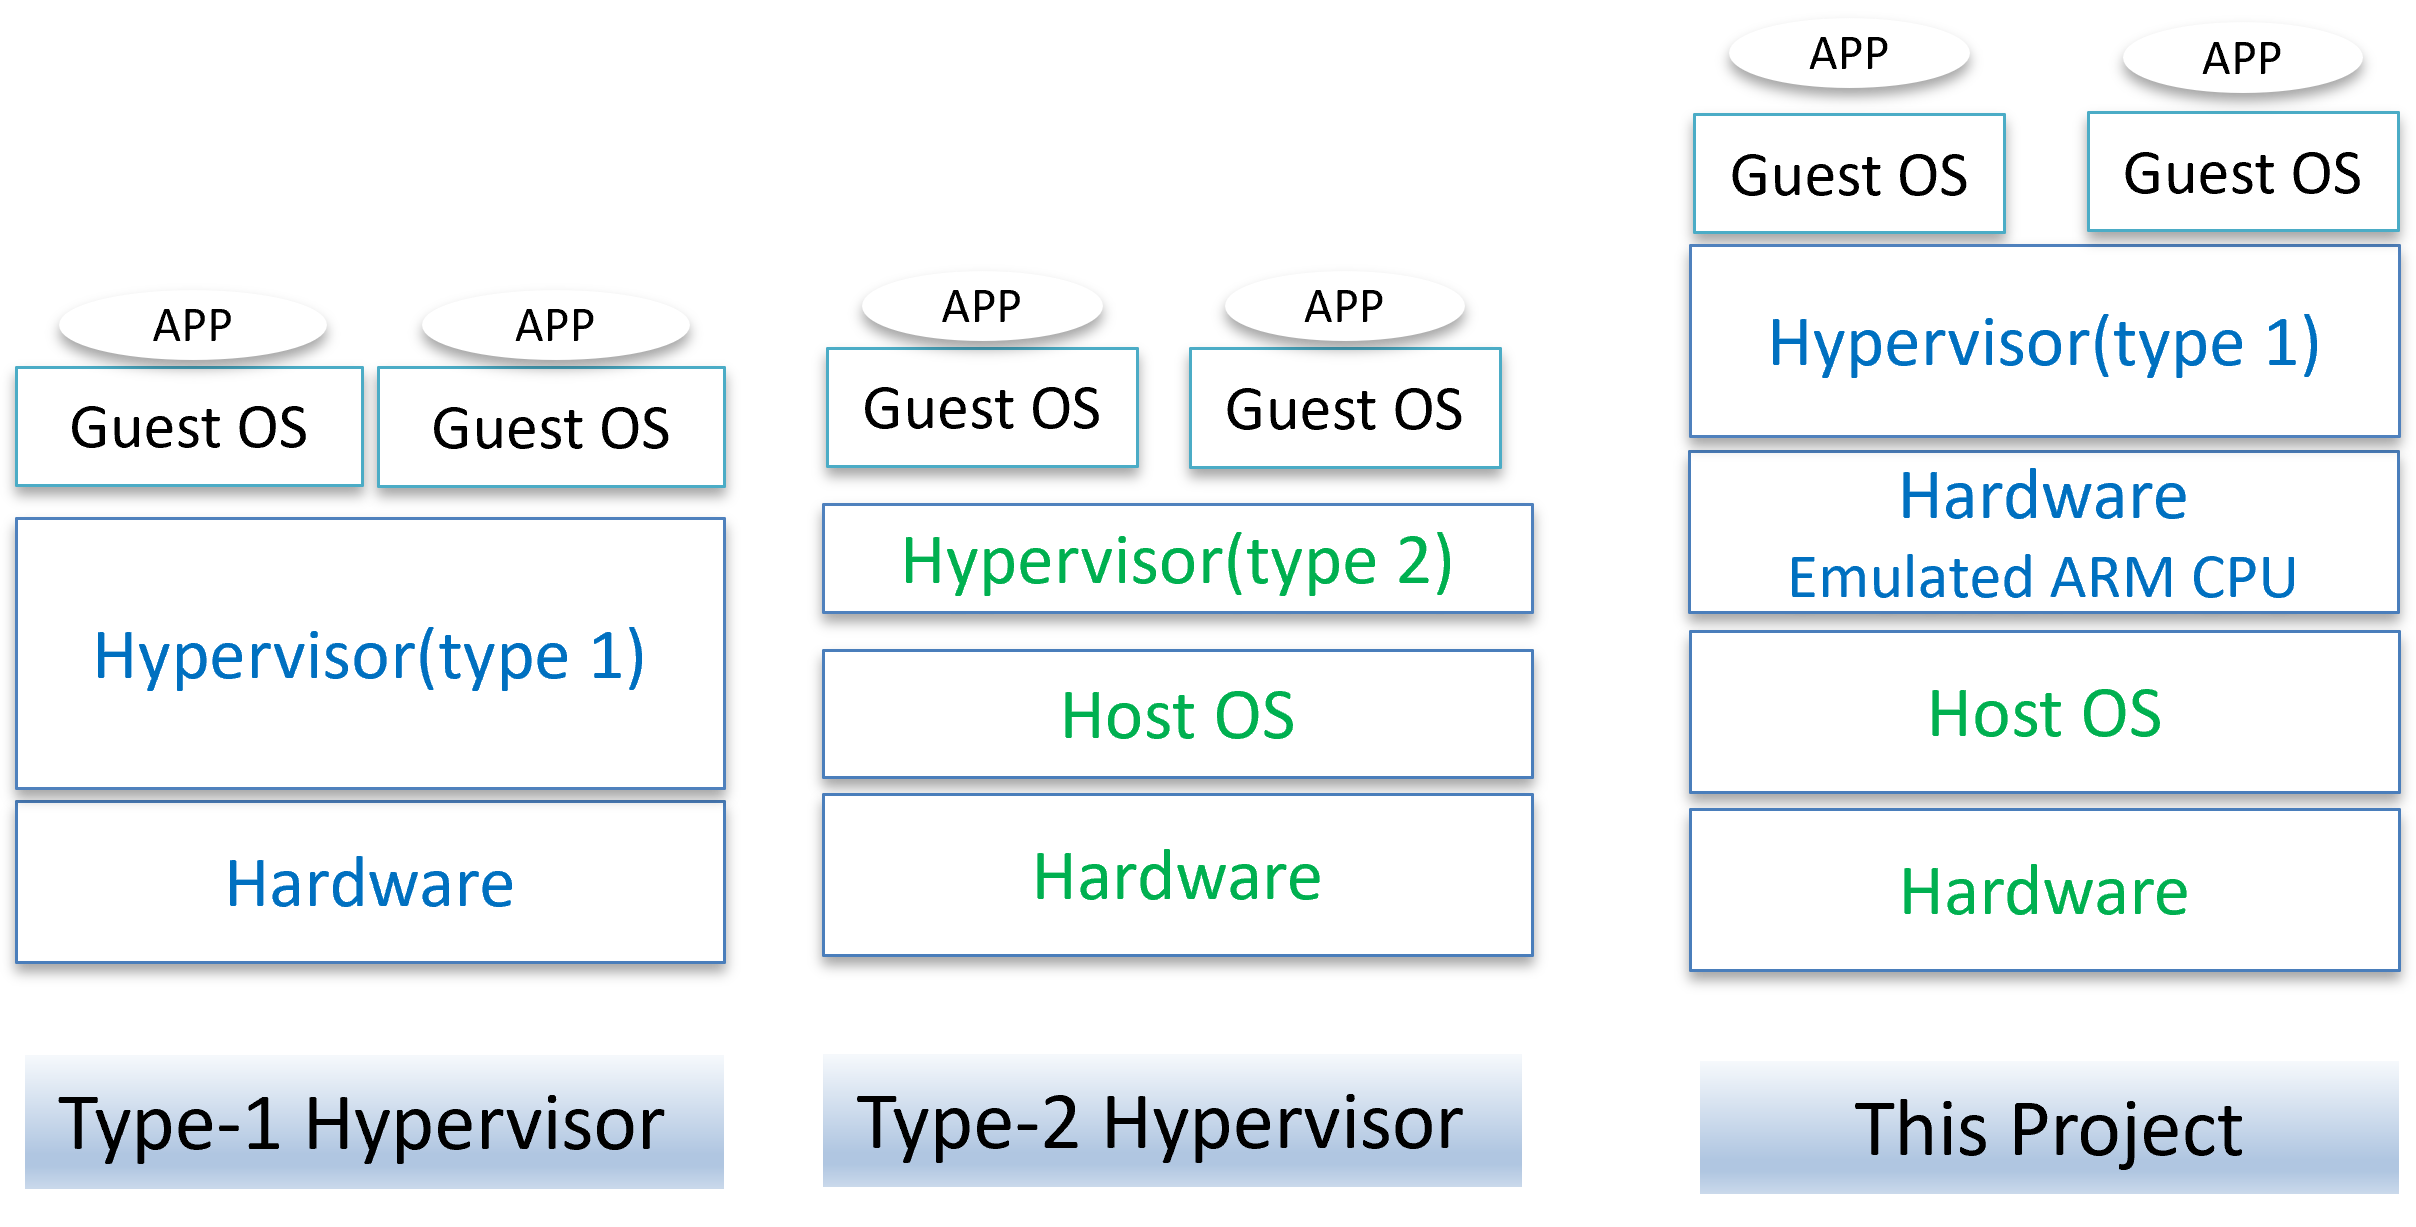
\includegraphics[width=\columnwidth]{images/type12_hyper.png}
  \caption{Type1, Type2 and this Project used Hypervisor}
  \label{fig:compare_hypervisor}
\end{figure}


Figure~\ref{fig:compare_hypervisor} illustrates the hypervisor architectures of Type-1 and Type-2 hypervisors compared to the structure used in this project. The hypervisor setup in this project differs significantly from conventional Type-1 and Type-2 hypervisors in both complexity and flexibility.

\paragraph{Type-1 Hypervisor:}
A Type-1 hypervisor, also known as a bare-metal hypervisor, runs directly on the underlying hardware. Both the hypervisor and its guest operating systems share the same architecture as the hardware (e.g., x86 or ARM). While this design offers high performance and direct hardware access, it depends entirely on the hardware platform.

\paragraph{Type-2 Hypervisor:}
A Type-2 hypervisor operates on top of a host operating system, relying on the host OS to manage hardware resources. Similar to Type-1 hypervisors, both the hypervisor and guest OSes must share the same architecture as the underlying hardware. This structure is easier to set up but adds overhead and remains tightly coupled to the hardware platform.

\paragraph{This Project's Hypervisor Architecture:}
In contrast, the hypervisor structure implemented in this project provides greater flexibility by decoupling the hypervisor and guest operating systems from the underlying hardware architecture. Using QEMU, the ARM CPU is emulated, enabling the Xen Type-1 hypervisor and guest OSes (ARM architecture) to run on an x86-based host machine. This hardware-independent design eliminates the architectural constraints imposed by conventional Type-1 and Type-2 hypervisors, allowing cross-platform testing and development.

\paragraph{Advantages of This Project's Architecture:}
The added complexity of this setup is justified by the increased flexibility it provides:
\begin{itemize}
    \item \textbf{Cross-Platform Compatibility:} By emulating the ARM CPU, this architecture allows the hypervisor and guest OSes to run on any hardware, regardless of the underlying architecture.
    \item \textbf{Hardware Independence:} Unlike conventional hypervisors, the virtualization stack does not depend on the hardware's native architecture, enabling secure and flexible experimentation in environments where physical ARM hardware is unavailable.
    \item \textbf{Enhanced Testing and Development:} This architecture is ideal for developing and testing secure applications that leverage TrustZone, as it provides a controlled and reproducible virtualized environment.
\end{itemize}

This project demonstrates that by combining QEMU, Xen, and OP-TEE, it is possible to create a highly versatile and secure virtualization stack that surpasses the constraints of traditional hypervisor architectures.


\subsection{QEMU: A System Emulator}
QEMU is a versatile system emulator widely used in research and development to emulate various architectures, including x86, ARM, MIPS, RISC-V, and more. It serves as a critical tool for enabling cross-platform development and testing without requiring physical hardware \cite{efficient_virtualization, partemu, qemu_fast_portable}. \cite{10.5555/1247360.1247401}

In the context of this project, QEMU plays a pivotal role by providing an ARM-emulated environment that supports the integration of ARM TrustZone with the Xen hypervisor. Its ability to emulate full systems, including CPUs, devices, kernels, and applications, makes it ideal for evaluating Trusted Execution Environments (TEEs) like OP-TEE. QEMU's system emulation mode allows the emulation of a complete computer system, including peripherals, enabling the virtual hosting of several virtual machines on a single physical host \cite{efficient_virtualization}.

QEMU operates in multiple modes:
\begin{itemize}
    \item \textbf{User-mode emulation:} This mode allows QEMU to execute individual Linux or Darwin/macOS programs compiled for different instruction sets. It translates system calls for endianness and architecture compatibility, making it a useful tool for cross-compilation and debugging.
    \item \textbf{System emulation:} In this mode, QEMU emulates an entire computer system, including its peripherals. This capability supports the execution of various guest operating systems, such as Linux, Windows, Solaris, and BSD, across architectures like ARMv7, ARMv8, x86, and more \cite{qemu_fast_portable}.
    \item \textbf{Hypervisor support:} QEMU can act as a Virtual Machine Manager (VMM) or as a device emulation back-end for virtual machines running under a hypervisor. When paired with a Kernel-based Virtual Machine (KVM) or hypervisors like Xen, it achieves near-native execution speeds while maintaining extensive emulation capabilities \cite{partemu}.
\end{itemize}

One of QEMU's core features is its use of Tiny Code Generator (TCG) to translate guest CPU instructions into equivalent host assembly instructions. This dynamic translation capability enables flexible and efficient execution of virtualized workloads, making QEMU an indispensable tool for developing and benchmarking systems that incorporate ARM TrustZone.

Through its robust emulation features and support for a variety of architectures and virtualization setups, QEMU provides the foundation for this project's exploration of secure and virtualized environments with ARM TrustZone.




\section{System Design: Introduction to the Virtualization Stack}

This section outlines the design and implementation of a virtualized environment to enable TrustZone-based applications on QEMU. we will explain how to enable a TrustZone-based application to run in a virtualized environment on QEMU in an X86 CPU. The process involves incrementally layering virtualization technologies, starting with the basic ARM CPU with TrustZone, then introducing the hypervisor to virtulize the TEE rich OS, and finally virtualizing the ARM CPU with QEMU. Below is a high-level overview of the stack:


\begin{itemize}
    \item TrustZone Application (via OP-TEE)
    \item Linux Guest OS
    \item Hypervisor (Xen)
    \item QEMU (emulates ARM CPU)
    \item AnyCPU (host OS)
\end{itemize}

We will explore each step in detail, showing how the system is built up layer by layer.

\subsection{Step 1: Bare Metal Machine. OS directly running on ARM CPU}

The first step is to show the basic setup where Linux OS runs directly on an ARM CPU that supports TrustZone. TrustZone provides a hardware-based isolation mechanism, dividing the CPU into two "worlds": the secure world (TrustZone) and the non-secure world (Linux). Here, Linux directly interacts with the ARM CPU, running in the non-secure world while TrustZone applications run in the secure world. This setup represents the simplest form of running Linux with TrustZone support.

\begin{figure}[ht]
  \centering
  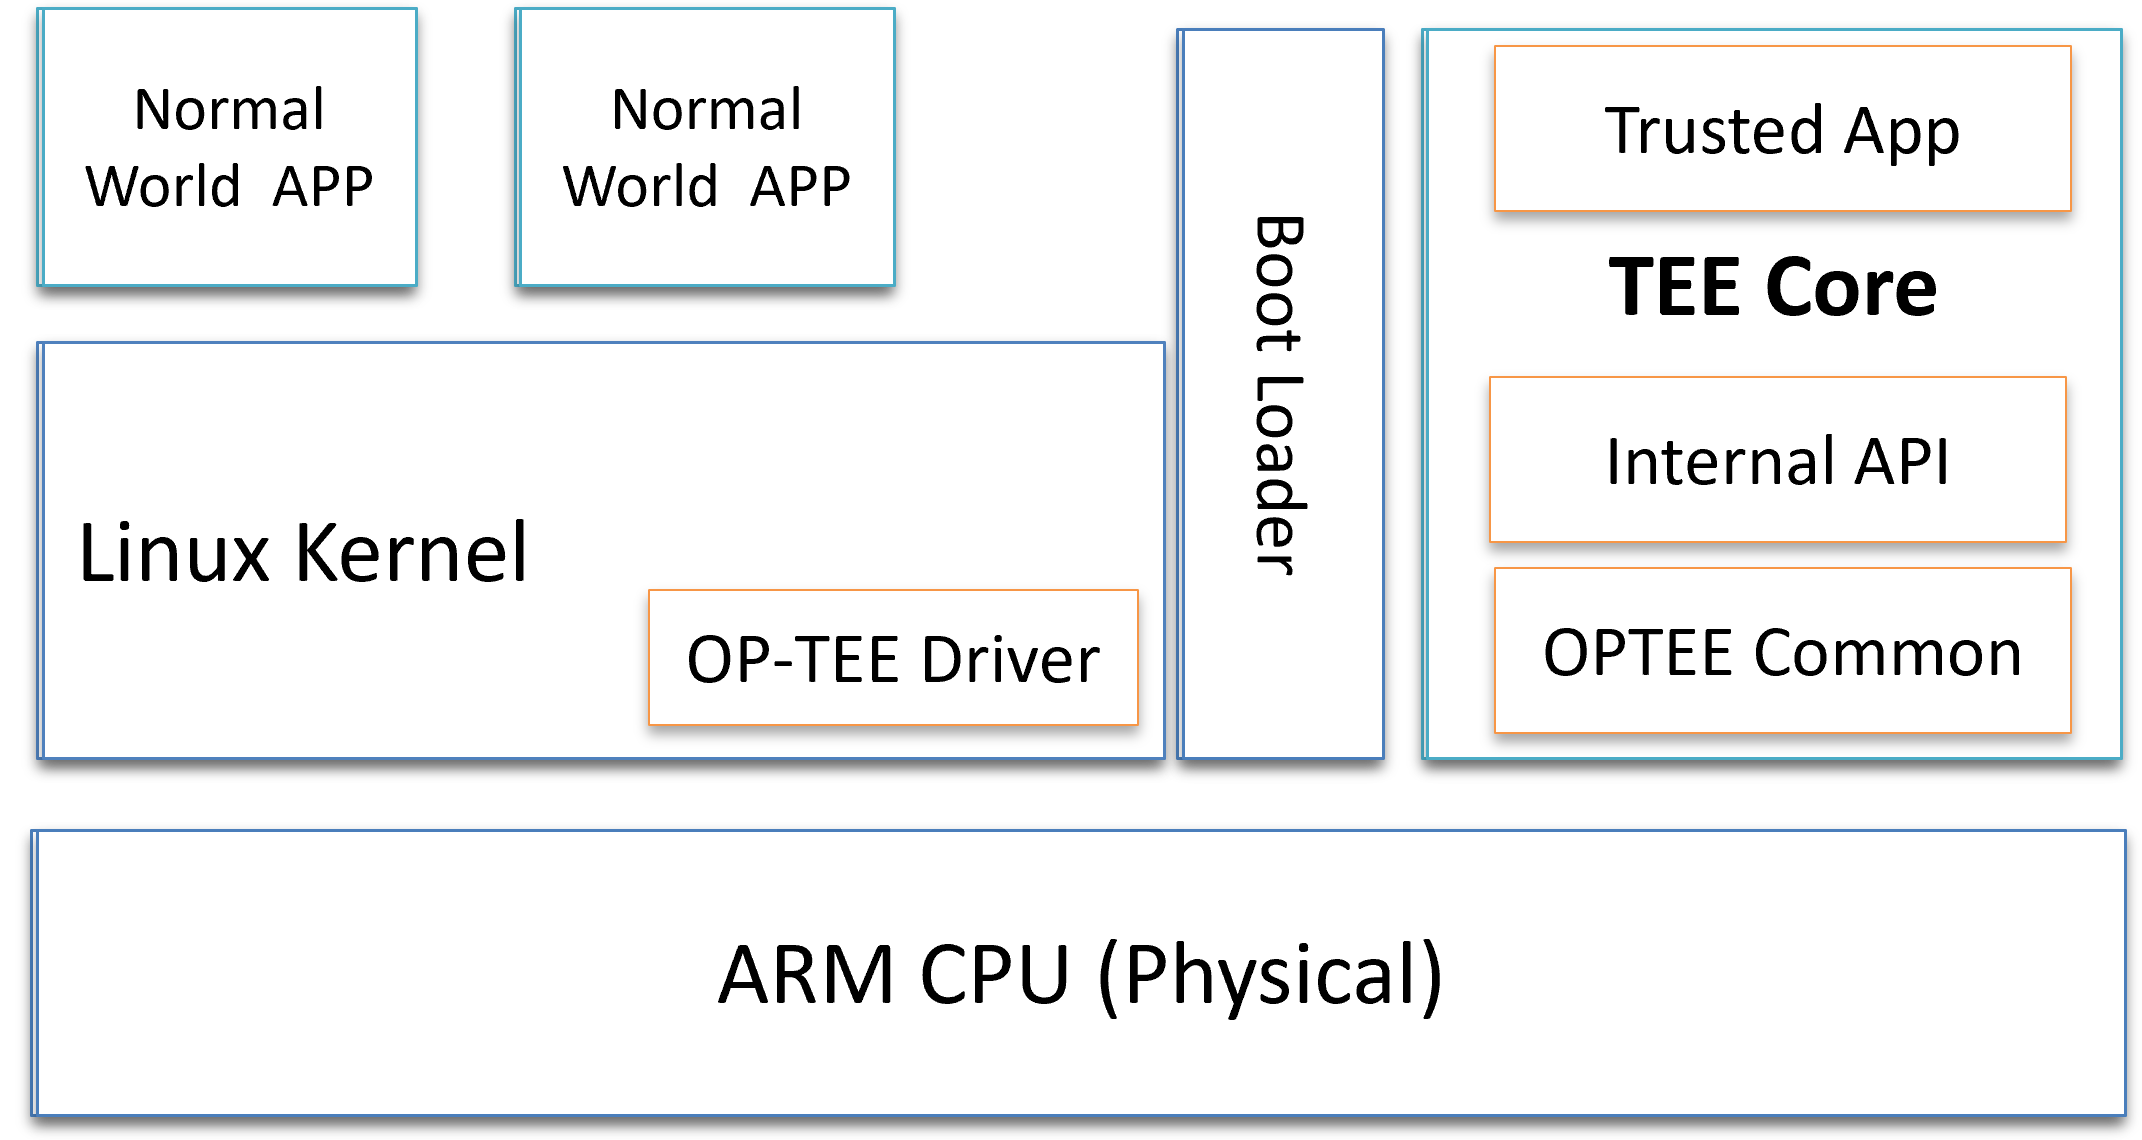
\includegraphics[width=\columnwidth]{images/1.png}
  \caption{ARM Trusted App, no virtualization}
  \label{fig:image_label}
\end{figure}



\subsection{Step 2: Virtualize the OS by introducing Hypervisor}
The next step involves introducing a hypervisor (in this case, Xen) to the system. The hypervisor provides a layer of abstraction, allowing multiple operating systems to run concurrently on the same hardware. In this scenario, Xen is installed on the ARM CPU, and Linux is virtualized into a guest operating system. The hypervisor ensures that the guest OSes are isolated from one another and the underlying hardware. This setup enables the secure TrustZone application to run alongside the virtualized Linux OS.

In this step, we introduce the concept of a hypervisor, which is critical to enabling the virtualization of the system. The hypervisor, in this case, Xen, runs directly on the ARM CPU and acts as a layer between the hardware and the operating systems (OSes) that need to run on top of it. 

In our configuration, we utilize Xen as a Type 1 hypervisor. It runs directly on the ARM hardware, which allows it to manage the system's resources and allocate them efficiently to virtual machines (VMs). The Xen hypervisor introduces the concept of domains: 
\begin{itemize}
    \item \textbf{Domain 0 (Dom0):} This is the privileged domain that has direct access to hardware resources and manages other domains. It typically runs a Linux-based OS, which is responsible for managing virtual devices and the overall virtualization environment.
    \item \textbf{Domain U (DomU):} These are the unprivileged domains or virtual machines that run on top of Dom0. Each DomU runs its own guest operating system, which in our case is a Linux OS. DomU does not have direct access to hardware, and its interactions with the hardware must go through Dom0 or the hypervisor.
\end{itemize}

Xen ensures that these domains are isolated from one another, preventing one compromised domain from affecting the others. This isolation is a critical feature of virtualization as it allows multiple guest OSes to run safely on the same hardware, without interference.



\begin{figure}[ht]
  \centering
  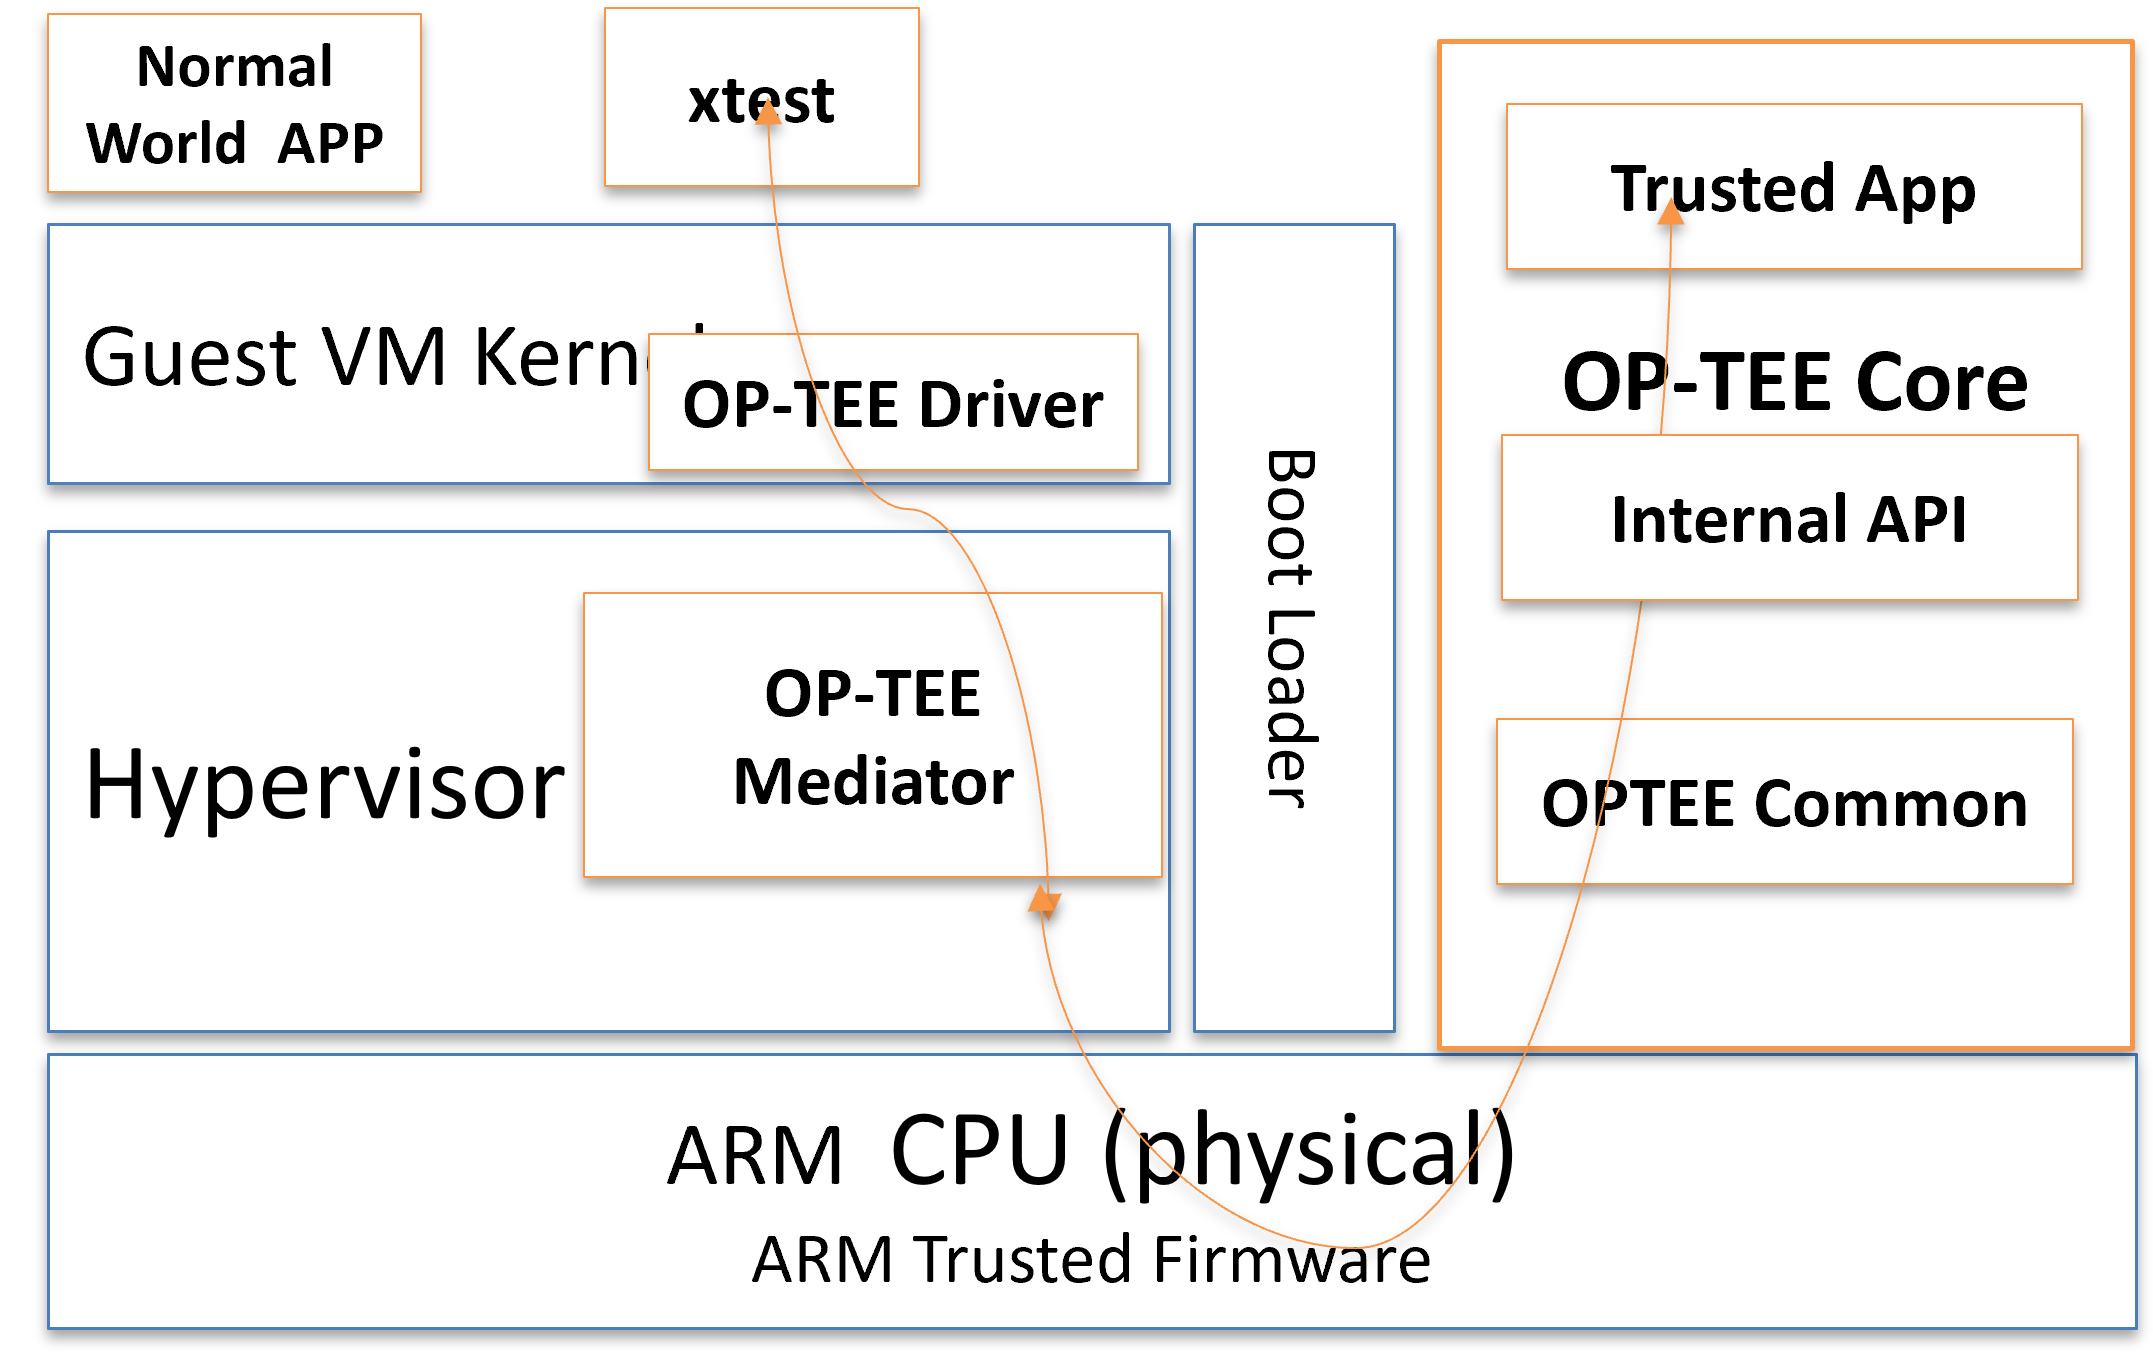
\includegraphics[width=\columnwidth]{images/2.png}
  \caption{Linux OS is virtualized by Xen hypervisor}
  \label{fig:image_label}
\end{figure}


\subsection{Step 3: Virtualizing the ARM CPU by QEMU}

The final step in the virtualization stack leverages QEMU to emulate the ARM CPU on a non-ARM machine, such as an x86-based host. QEMU provides full system emulation, enabling the ARM architecture to function independently of physical hardware. This setup allows the Xen hypervisor to run on a virtualized ARM CPU, which, in turn, manages guest operating systems and facilitates TrustZone functionality.

In this configuration:
\begin{itemize}
    \item \textbf{TrustZone Application:} Securely runs in the ARM TrustZone, isolated from the non-secure world.
    \item \textbf{Linux Guest OS:} Operates in the non-secure world on the virtualized ARM hardware.
    \item \textbf{Hypervisor (Xen):} Provides the virtualization layer, ensuring resource isolation and security.
    \item \textbf{QEMU (ARM CPU Emulator):} Emulates the ARM architecture, enabling the stack to run on a non-ARM host.
    \item \textbf{Host OS (AnyCPU):} Supplies the physical resources for virtualization and emulation.
\end{itemize}

\begin{figure}[ht]
  \centering
  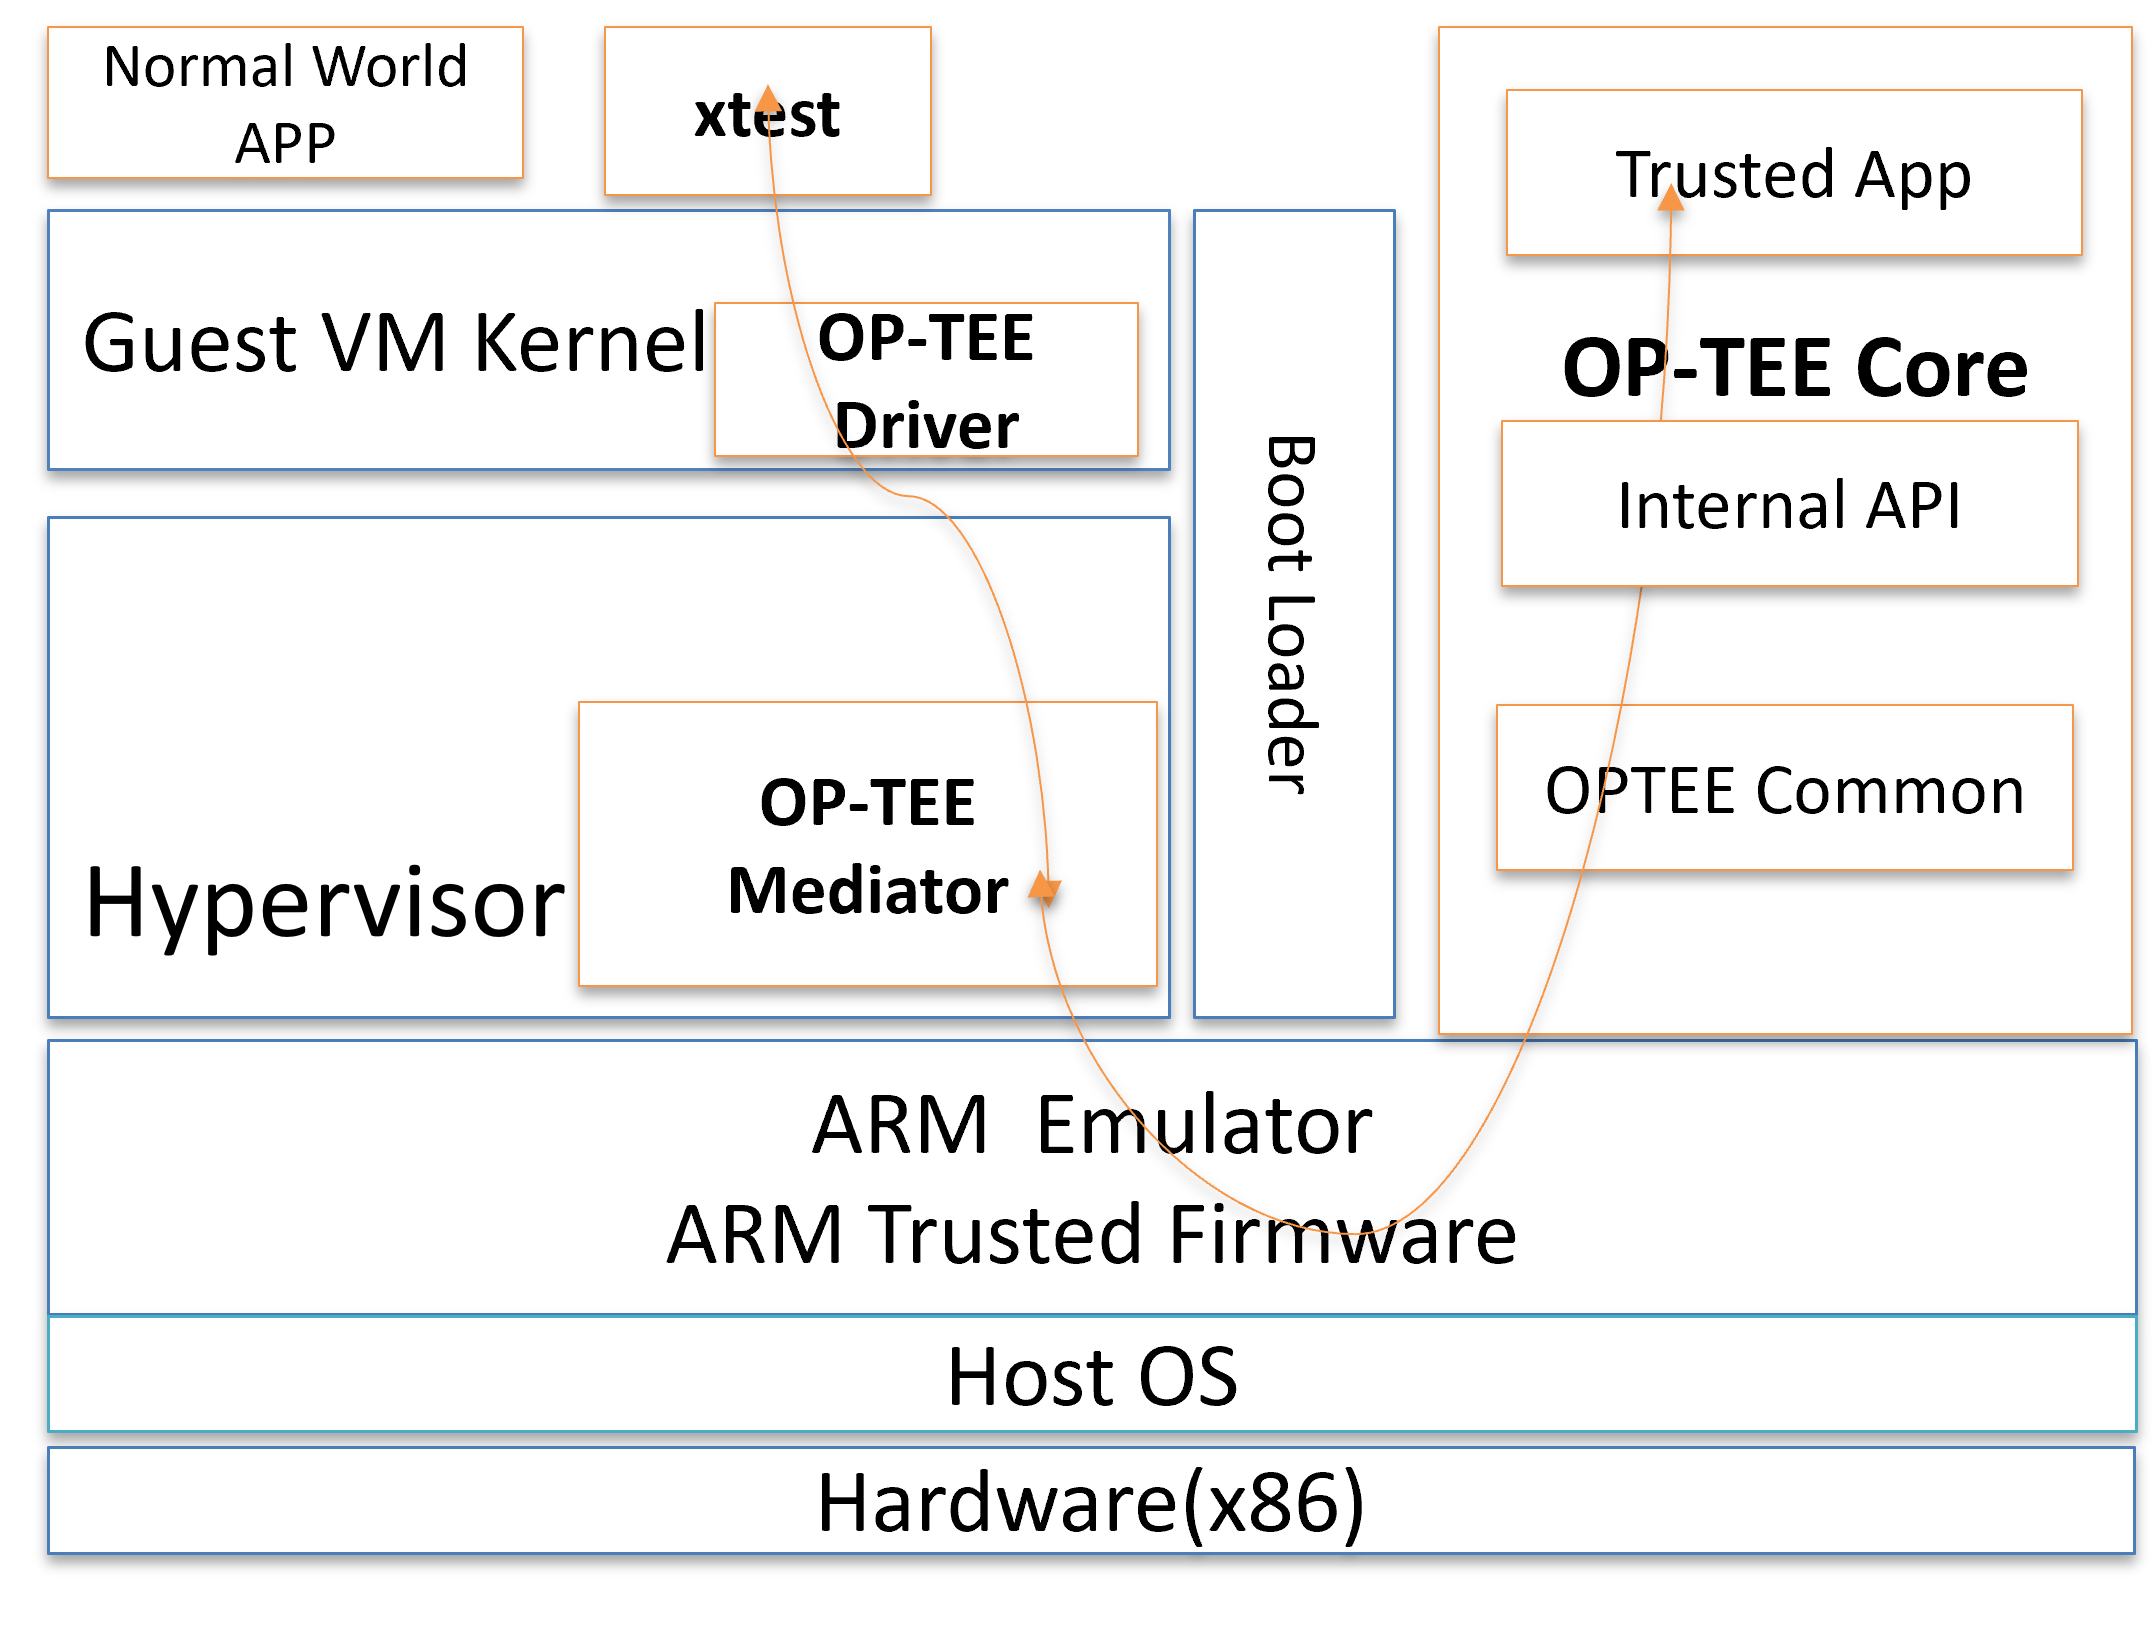
\includegraphics[width=\columnwidth]{images/3.png}
  \caption{Final Virtualization Stack. ARM Processor is virtualized by QEMU}
  \label{fig:virtual_stack}
\end{figure}

\subsection{Recap}
In summary, the virtualization stack was built incrementally to enable TrustZone applications in a flexible and secure environment:
\begin{itemize}
    \item \textbf{Step 1: Bare-Metal Setup:} Linux was configured to run directly on an ARM CPU with TrustZone support, establishing the foundational hardware-based isolation between the Secure World and Non-Secure World.
    \item \textbf{Step 2: Virtualization with Xen:} The Xen hypervisor was introduced to virtualize the ARM CPU, enabling the concurrent execution of multiple isolated guest operating systems.
    \item \textbf{Step 3: Emulation with QEMU:} QEMU was employed to emulate the ARM CPU, allowing the entire stack to operate seamlessly on non-ARM hardware, such as x86-based platforms.
\end{itemize}

This step-by-step approach integrates TrustZone with virtualization and emulation technologies, showcasing a scalable framework for testing, debugging, and researching secure applications in virtualized embedded systems. By combining the strengths of QEMU and Xen, the stack achieves both hardware independence and robust isolation, making it a versatile tool for advancing TrustZone-based research.



% \section{Evaluation}
% \section{Conclusion \& Discussion}
\section{Implementation}

This section describes the implementation of the virtualization stack to enable TrustZone-based applications. 

The implementation of the virtualization stack primarily followed the guidance provided by Denis Obrezkov for setting up Xen, QEMU, and Linux configurations \cite{obrezkov2019xen}. However, our work leverages the most up-to-date software versions to ensure compatibility and improved functionality. For the Trusted Execution Environment (TEE) components, we relied on the official OP-TEE documentation to ensure proper integration and configuration of secure world operations \cite{optee_docs}.

\subsection{System Components}
Our implementation relies on the following primary components:
\begin{itemize}
  \item \textbf{Trusted Execution Environment:} Trusted Application Benchmark (xtest) in Normal World, along with OP-TEE Core within Secure World to manage and execute trusted applications.
    \item \textbf{Hypervisor:} Xen hypervisor with experimental support for OP-TEE, providing robust virtualization capabilities.
    \item \textbf{ARM Emulator:} QEMU configured with ARM virtualization extensions to emulate the ARM CPU and facilitate the virtualization stack on x86-based hardware.
    \item \textbf{Guest Operating Systems:} Linux kernel, compiled for both secure and non-secure environments, running as guest OSes.
    \item \textbf{Bootloader:} U-Boot to initialize the system and load the Xen hypervisor and guest operating systems.
    \item \textbf{Utility Tools:} BusyBox for creating a lightweight root filesystem for the guest Linux environments.
\end{itemize}


The key software components used in our implementation include: 

\begin{itemize}
  \item \textbf{OP-TEE:} Version 4.3.0

  \item \textbf{Xen:} Version 4.18.3
  \item \textbf{QEMU:} Version 9.1.0

    \item \textbf{BusyBox:} Version 1.37.0
    \item \textbf{Linux Kernel:} Version 6.1.18

    \item \textbf{U-Boot:} Version 2024.07


\end{itemize}



\subsection{Role of the Hypervisor in OP-TEE Integration}

The hypervisor plays a critical role in facilitating secure interaction between virtual machines (VMs) and the Trusted Execution Environment (TEE) provided by OP-TEE. VMs cannot directly call OP-TEE due to several virtualization and security challenges, including the lack of physical address awareness, the need for OP-TEE to track VM creation and destruction, and the requirement to identify which VM is making a request. Additionally, the hypervisor ensures memory isolation, preventing one VM from referencing another VM's memory when interacting with OP-TEE. By addressing these challenges, the hypervisor enables secure and efficient integration of OP-TEE into the virtualized environment. OP-TEE need to track life cycle of VMs. So it provides two special
calls: 
\begin{itemize}
  \item \texttt{OPTEE\_SMC\_VM\_CREATED VMID}
  \item \texttt{OPTEE\_SMC\_VM\_DESTROYED VMID}
\end{itemize}
Hypervisor informs OP-TEE about VM creation or destruction by issuing above SMCs.



\subsection{OP-TEE Virtualization Support: XEN TEE Mediator}

OP-TEE provides experimental support for virtualization, allowing a single OP-TEE instance to securely execute Trusted Applications (TAs) from multiple virtual machines (VMs). This is achieved by isolating VM-specific states within OP-TEE, ensuring that operations from one VM cannot affect another. Such isolation is critical for maintaining the integrity and security of Trusted Execution Environments (TEEs) in virtualized systems.

In a virtualized setup, OP-TEE relies heavily on the hypervisor to mediate interactions between VMs and the TEE. The hypervisor is responsible for:
\begin{itemize}
    \item Identifying which VM is making a request to OP-TEE.
    \item Informing OP-TEE about the creation and destruction of VMs to manage secure resources effectively.
    \item Translating Intermediate Physical Addresses (IPAs) used by VMs into Physical Addresses (PAs) required by OP-TEE, as OP-TEE cannot process IPAs directly.
\end{itemize}

To support these functions, Xen includes a specialized component called the "TEE Mediator." This mediator ensures secure communication between VMs and OP-TEE while maintaining isolation and proper address translations.

To enable OP-TEE support in Xen, two configuration methods can be used: interactive menu-based configuration and non-interactive command-line configuration.

\paragraph{Interactive Menu Configuration:}
\begin{enumerate}
    \item Navigate to the Xen source directory.
    \item Run the \texttt{make menuconfig} command to access the Xen configuration menu.
    \item Enable the \texttt{OPTEE} option under the "Architecture Features" section.
    \item Ensure that the "TEE mediators" option is also enabled.
    \item Save the configuration and exit the menuconfig tool.
    \item Compile and install Xen with the updated configuration.
\end{enumerate}

The specific path in the Xen interactive menu for enabling OP-TEE support is:
\texttt{Xen/arm 4.18.3 configuration -> Architecture Features -> TEE mediators -> Enable OP-TEE mediator (UNSUPPORTED)}.

\paragraph{Non-Interactive Command-Line Configuration:}
Alternatively, the configuration can be performed directly by modifying the Xen `.config` file. The following changes enable OP-TEE support: edit the \texttt{xen/.config} file and update the following options:

\begin{lstlisting}[language=make, caption=Enable OP-TEE Support in Xen Configuration]
# Xen configuration file: xen-4.18.3/xenxen/.config

CONFIG_TEE=y       # Enable Trusted Execution Environment (TEE) support
CONFIG_OPTEE=y     # Enable OP-TEE mediator support
\end{lstlisting}


By enabling OP-TEE support through either method, Xen becomes capable of securely managing interactions between VMs and the Trusted Execution Environment. This setup is critical for testing and deploying TrustZone-based applications in virtualized environments.


\subsection{OP-TEE Linux Kernel Support}
The OP-TEE driver in the guest VM kernel is essential for enabling secure communication between the guest operating system and the Trusted Execution Environment (TEE) provided by OP-TEE. In a virtualized environment, guest VMs rely on the hypervisor to manage hardware resources, but direct access to TrustZone features is not inherently available to these VMs. The OP-TEE driver acts as an intermediary, allowing guest applications to issue secure requests to OP-TEE. This integration ensures that security-critical operations, such as cryptographic computations and secure storage, can be performed in the TEE without exposing sensitive data to the untrusted hypervisor or other guest VMs. Furthermore, the driver abstracts the complexity of managing TrustZone interactions, enabling seamless use of OP-TEE services within the virtualized ecosystem, thus enhancing the security capabilities of the guest VM.

To enable the OP-TEE driver in the guest VM kernel, the configuration must be set within the Linux kernel menuconfig tool. The specific path to access and configure this driver is:
\texttt{.config - Linux/x86 6.1.18 Kernel Configuration -> Device Drivers -> Trusted Execution Environment Support}

The following commands and configurations are applied via the command line:
\begin{lstlisting}[language=make, caption=Enabling OP-TEE in the Linux Kernel Configuration]
 
  # Linux configuration file: linux-6.1.18/.config
      CONFIG_XEN=y          # Enable Linux Kernel support for XEN
      CONFIG_XEN_DOM0=y     # Support Linux running as a Xen Dom0 guest

      
      CONFIG_TEE=y          # Enable Linux Kernel support for Trusted Execution Environment (TEE) 
      CONFIG_OPTEE=y        # Enable Linux Kernel support for OP-TEE
\end{lstlisting}


\section{Benchmark Performance Analysis}

The \textit{xtest} benchmark suite was executed to evaluate the performance of the OP-TEE Trusted Execution Environment (TEE) in the context of our virtualization stack. The results provide critical insights into the feasibility of integrating OP-TEE with Xen and QEMU to enable secure applications in virtualized embedded systems.

\subsection{Results Overview}
The benchmark suite completed 24 subtests successfully, with no failures, indicating the stability of the OP-TEE environment within the virtualized setup. Key observations include:

\begin{itemize}
    \item \textbf{Trusted Storage Performance:} Write operations were efficient for smaller data sizes (up to 28.57 kB/s for 1 KB), but performance decreased significantly for larger files (17.09 kB/s for 1 MB). Read operations consistently outperformed writes, peaking at 250 kB/s for 2 KB, but dropped to 134.95 kB/s for 1 MB.
    \item \textbf{Cryptographic Performance:} 
    \begin{itemize}
        \item SHA1 achieved a mean speed of 0.48 MiB/s, while SHA256 performed significantly better at 2.22 MiB/s, demonstrating the TEE's capability to handle secure hash operations efficiently.
        \item AES encryption showed stable performance, with ECB mode achieving 0.61 MiB/s and CBC mode slightly higher at 0.63 MiB/s.
    \end{itemize}
    \item \textbf{Rewriting Data:} Rewrites exhibited a similar trend to writes, with small data sizes performing efficiently but a sharp decline in speed for larger files.
\end{itemize}

\subsection{Project-Specific Insights}
The benchmark results align closely with the objectives of this project, demonstrating the viability of integrating OP-TEE with a Xen-based virtualized environment on QEMU. Key takeaways include:

\begin{itemize}
    \item \textbf{Secure Storage Limitations:} While the TEE effectively secures storage operations, the performance degradation for larger data sizes highlights potential bottlenecks in scenarios involving high-throughput applications. This aligns with the project's focus on testing and identifying limitations in the current implementation.
    \item \textbf{Cryptographic Workloads:} The strong performance in SHA and AES benchmarks validates OP-TEE's suitability for handling cryptographic tasks within a secure environment. This result is significant for the project's goal of evaluating the TEE's ability to support security-critical applications in a virtualized setup.
    \item \textbf{Single-VM Context:} The benchmarks confirm the functional stability of OP-TEE in the current single-VM configuration. However, the project's requirement to support multiple VMs presents a challenge, as performance implications for multi-VM setups remain unexplored.
\end{itemize}

\subsection{Implications for Virtualized Embedded Systems}
The results underscore the strengths and challenges of leveraging OP-TEE in virtualized environments:
\begin{itemize}
    \item \textbf{Strengths:} Cryptographic operations and secure isolation were efficiently managed, indicating that OP-TEE can provide robust security services within a virtualized system.
    \item \textbf{Challenges:} The performance decline for large-scale storage operations and the absence of multi-VM support reveal critical areas for improvement to meet production-level demands.
\end{itemize}

Overall, the benchmarks demonstrate that the integration of OP-TEE with Xen and QEMU provides a secure and functional foundation for virtualized embedded systems. Future work will focus on addressing identified limitations to scale this solution for multi-VM environments, aligning with the project's long-term objectives.


\section{Challenges}

During the implementation of the virtualization stack, several challenges were encountered. While some issues stemmed from real mistakes in the original tutorial \cite{obrezkov2019xen}, others were due to differences introduced by software updates, as we used significantly newer versions of Xen, QEMU, Linux, U-Boot, and OP-TEE. These updates, spanning over five years, led to changes in software behavior, configuration options, and compatibility requirements, necessitating adjustments and debugging to align with the updated software ecosystem.


\subsection{BusyBox Hardware Acceleration Compatibility}

When compiling BusyBox for use in a virtualized environment like QEMU with Xen, it is essential to disable hardware acceleration (HWA) features. This is because virtualized environments typically do not provide direct access to hardware acceleration, such as NEON on ARM platforms. Enabling HWA during compilation can result in build failures or runtime issues due to the lack of support for hardware-accelerated instructions in emulated environments.

To ensure compatibility, HWA must be explicitly disabled in the BusyBox configuration, aligning the build with the constraints of the virtualized environment.

To compile BusyBox without hardware acceleration, follow these steps:

\begin{lstlisting}[language=bash, caption=Solution to HWA Fault]
# Disable Hardware Acceleration in configuration
sed -i 's/CONFIG_SHA1_HWACCEL=y/CONFIG_SHA1_HWACCEL=n/' .config
sed -i 's/CONFIG_SHA256_HWACCEL=y/CONFIG_SHA256_HWACCEL=n/' .config
\end{lstlisting}


By disabling hardware acceleration, the compiled BusyBox binaries rely solely on software implementations. This ensures compatibility and stable performance in virtualized environments, avoiding potential issues with unsupported hardware features.



\subsection{BusyBox Compilation Failure with Traffic Control Utility}
During the compilation of BusyBox, a issue was encountered when enabling support for the \texttt{tc} (traffic control) utility. The problem arises due to the removal of the \texttt{CBQ (Class-Based Queuing)} feature from the Linux kernel. Specifically, the kernel headers no longer define the constant \texttt{TCA\_CBQ\_MAX}, which is referenced in the BusyBox source code.

\begin{lstlisting}[language=bash, caption=Failure on compile BusyBox]
networking/tc.c: In function cbq_print_opt:
networking/tc.c:236:27: error: TCA_CBQ_MAX undeclared
 (first use in this function); did you mean TCA_CBS_MAX?
  236 |         struct rtattr *tb_TCA_CBQ_MAX+1_;
      |                           ^~~~~~~~~~~
      |                           TCA_CBS_MAX
\end{lstlisting}

\paragraph{Root Cause:}The \texttt{tc} utility relies on kernel features like CBQ for traffic shaping and queuing. With these features deprecated and subsequently removed from newer kernel versions, the corresponding BusyBox code referencing \texttt{TCA\_CBQ\_MAX} cannot compile.

To resolve this, \texttt{tc} support needs to be disabled in BusyBox's configuration file (\texttt{.config}). This can be done using the following command:

\begin{lstlisting}[language=bash, caption=Solution to Disable Traffic Control ]
sed -i 's/CONFIG_TC=y/CONFIG_TC=n/' .config
\end{lstlisting}

Disabling \texttt{tc} is a practical workaround if traffic control functionality is not required, this change prevents the compilation of the \texttt{tc} utility, avoiding the error.





\subsection{QEMU stuck on loading unsupported GPIO module}
QEMU with Xen Stuck on Loading Linux as \texttt{dom0}

A challenge was encountered when running QEMU with Xen to start Linux as \texttt{dom0}. The system would get stuck during the boot process due to issues related to the Advanced Microcontroller Bus Architecture (AMBA) compliant controller. This problem manifested in the output as follows:

\begin{lstlisting}[language=bash, caption=QEMU stuck on unsupported GPIO module]
# Start the QEMU virtual emulation
$ qemu-system-aarch64  -machine virt,gic_version=3 -machine virtualization=true \
  -cpu cortex-a57 -machine type=virt -m 4096 -smp 4 -bios u-boot.bin \
  -device loader,file=xen,force-raw=on,addr=0x49000000 \
  -device loader,file=Image.gz,addr=0x47000000 \
  -device loader,file=virt-gicv3.dtb,addr=0x44000000 \
  -device loader,file=rootfs.img.gz,addr=0x42000000 \
  -nographic -no-reboot \
  -chardev socket,id=qemu-monitor,\
   host=localhost,port=7777,server,nowait,telnet \
  -mon qemu-monitor,mode=readline

... [Truncated output] ...

### XEN booting up, but stuck at loading DOM0 ###
(XEN) d0v1: vGICR: SGI: unhandled word write 0x000000ffffffff to ICACTIVER0
\end{lstlisting}

The process would hang indefinitely, requiring manual intervention to terminate.

\paragraph{Root Cause:}The problem is linked to the ARM \texttt{PL061} GPIO module, which is part of the AMBA controller. Xen attempts to manage this hardware during boot, but it lacks full support for the \texttt{PL061} module in the current configuration. As a result, Xen gets stuck in an unhandled state.

The solution involves disabling the \texttt{PL061} controller in the device tree. This prevents Xen from trying to initialize unsupported hardware during the boot process. This can be achieved with the following steps:

\begin{lstlisting}[language=bash, caption=Solution to QEMU stuck]
dtc -I dtb -O dts virt-gicv3.dtb > virt-gicv3.dts
sed 's/compatible = "arm,pl061.*/status = "disabled";/g' virt-gicv3.dts > virt-gicv3-edited.dts
dtc -I dts -O dtb virt-gicv3-edited.dts > virt-gicv3.dtb
\end{lstlisting}

This procedure modifies the device tree to disable the incompatible \texttt{PL061} controller, allowing the system to proceed past the stuck state.

After applying these changes, QEMU successfully boots Linux as \texttt{dom0} under Xen without hanging. This solution provides a temporary workaround for environments where the \texttt{PL061} module is unnecessary or unsupported.




\subsection{Launching QEMU with Xen and Two Linux Instances}

This challenge involves configuring QEMU to run Xen and boot two Linux instances (\texttt{dom0} and \texttt{domU1}). The procedure requires careful memory and device tree setup due to changes in the size of Linux images in newer releases.

\paragraph{QEMU Launch Command}

The following command initializes QEMU with Xen, two Linux kernels, and their corresponding root file systems:

\begin{lstlisting}[language=bash, caption=Designed Device Layout]
qemu-system-aarch64 \
    -machine virt,gic_version=3 \
    -machine virtualization=true \
    -cpu cortex-a57 \
    -machine type=virt \
    -m 4096 \
    -smp 4 \
    -bios u-boot.bin \
    -device loader,file=xen,force-raw=on,addr=0x50000000 \
    -device loader,file=Image,addr=0x47000000 \
    -device loader,file=Image,addr=0x53000000 \
    -device loader,file=virt-gicv3.dtb,addr=0x44000000 \
    -device loader,file=rootfs.img.gz,addr=0x42000000 \
    -device loader,file=rootfs.img.gz,addr=0x58000000 \
    -mon qemu-monitor,mode=readline
\end{lstlisting}

% \subsubsection{Key Insight: Adapting to Larger Linux Images}

The size of the compiled Linux guest OS has increased in newer releases compared to the versions used in older tutorials. This increase can result in a \texttt{FDT\_ERR\_NOSPACE} error during boot due to insufficient space in the Flattened Device Tree (FDT).

U-Boot may failed with some error like this due to the larger image size.
\begin{lstlisting}[language=bash, caption=U-Boot error due to different image size]
  libfdt fdt_setprop(): FDT_ERR_NOSPACE
  chosen {
  riscv,kernel-start = <0x00000000 0x80200000>;
  };
\end{lstlisting}


To resolve this, it's necessary to include the \texttt{fdt resize} command before certain FDT modifications. This step ensures that the FDT can accommodate larger configurations.

% \subsubsection{U-Boot Configuration}

Below is the updated U-Boot configuration sequence:

\begin{lstlisting}[language=bash, caption=Solution to U-Boot error]
setenv xen_bootargs 'dom0_mem=512M'
fdt addr 0x44000000
<truncated>

# resize fdt to accommodate the real image size
fdt resize
fdt mknod /chosen/domU1 module@1
<truncated>
\end{lstlisting}


The key takeaway is that modern Linux kernels and images are significantly larger than their predecessors. This necessitates the use of \texttt{fdt resize} to prevent FDT errors and ensure a smooth boot process.

\section{Limitation}

At the current stage of the project, the OP-TEE feature is limited to supporting a single virtual machine (VM). While the project requirements specify the need to enable OP-TEE across two VMs, the following limitations were encountered:

\textbf{Single-VM Support in OP-TEE:} The current implementation of OP-TEE is designed to handle Trusted Applications (TAs) for a single VM. Extending this functionality to multiple VMs requires significant modifications and is not directly supported by the existing tutorials or configurations.


These limitations underscore the challenges of scaling OP-TEE for multi-VM setups and highlight areas for further development to meet the project’s requirements.


\section{Future Work}

One promising direction for future work is to combine the OP-TEE tutorial with the multi-VM setup outlined in the Xen wiki tutorial to enable support for multiple virtual machines (VMs). This enhancement would simulate a more realistic production environment, where multiple VMs can securely interact with a single OP-TEE instance.

However, achieving this goal requires addressing several challenges. Notably, OP-TEE has certain hardcoded configurations, such as the memory loading address for the secure image. Modifying these settings to accommodate multiple VMs demands additional effort and a deeper understanding of both OP-TEE's architecture and the Xen hypervisor's virtualization mechanisms. Overcoming these limitations would pave the way for advanced research into secure multi-VM environments using OP-TEE and Xen.



\section{Conclusion}

This project successfully implemented a virtualization stack integrating OP-TEE with the Xen hypervisor and QEMU emulator to evaluate the feasibility of enabling Trusted Execution Environment (TEE) functionality in a virtualized embedded system. The results from the \textit{xtest} benchmarks demonstrated the stability and performance of OP-TEE within a single-VM setup, validating its capability to securely handle cryptographic and storage operations.

However, the project also highlighted key limitations, including the lack of multi-VM support and performance bottlenecks for large-scale trusted storage operations. These findings underscore the need for further optimization and development to address scalability challenges and enhance the usability of OP-TEE in production environments.

Despite these challenges, this work provides a solid foundation for future research into secure virtualization. The integration of OP-TEE with Xen and QEMU not only demonstrates the viability of deploying TEEs in virtualized setups but also identifies critical areas for improvement. Future efforts will focus on extending support to multiple VMs and refining secure storage mechanisms to better meet the demands of real-world applications.

This project contributes to advancing the field of secure embedded systems, offering insights into the integration of hardware-based security technologies with modern virtualization platforms.



\bibliographystyle{ACM-Reference-Format}
\bibliography{references}

\end{document}
\endinput